
% Original template by Andrew G. West - prop_spec.tex
% Document by Cris Feo and Ben Perez
% Main LaTeX file for CIS400/401 Project Proposal Specification
%

	%	% AW - Ordinarily we'd begin by specifying some broad document properties like font-size, page-size, margins, etc. -- We have done this (and much more) for you by creating a 'style file', which the 'documentclass' command references.
\documentclass[]{sig-alternate}
 
	% AW - These 'usepackage' commands are a way of importing additional LaTeX styles and formattings that aren't part of the 'standard library'
\usepackage{mdwlist}
\usepackage{url}

\begin{document} 

	% AW - We setup the parameters to our title header before 'making' it.
\title{Semi-Supervised Wikipedia Category Suggestion}
\subtitle{}
\numberofauthors{4}
\author{
	\alignauthor Benjamin Perez \\ \email{bperez@seas.upenn.edu} \\ Univ. of Pennsylvania \\ Philadelphia, PA
	\alignauthor Cristoforo Feo \\ \email{cfeo@seas.upenn.edu}   \\ Univ. of Pennsylvania \\ Philadelphia, PA
\and
	\alignauthor Andrew G. West \\ \email{westand@cis.upenn.edu} \\ Univ. of Pennsylvania \\ Philadelphia, PA
	\alignauthor Insup Lee      \\ \email{lee@cis.upenn.edu}     \\ Univ. of Pennsylvania \\ Philadelphia, PA
}
\date{}
\maketitle


	% AW - Next we write out our abstract -- generally a two paragraph maximum, executive summary of the motivation and contributions of the work.
\begin{abstract}
\textit{In 2005 Wikipedia implemented a category system for the purposes of facilitating navigation throughout the site. Since then, it has grown to 1.5 million categories covering over four million articles. Currently, all categorization of articles on Wikipedia is done by human editors---a task which involves an enormous amount of repetitive work.}

\textit{This paper proposes building an automated system that suggests missing category-article links to editors through a browser-based user-interface. This system will utilize the existing corpus of human-categorized articles, as well as available metadata, to provide a ranked list of suggested categorizations. All suggested categorizations are subject to final approval or rejection by a human editor.}
\end{abstract}


\section{Introduction}
\label{sec:intro}
Fundamentally, Wikipedia consists of a number of content pages, or articles, and a series of categories to which articles might be linked. Categories may have sub categories and pages may belong to several different categories. In a traditional knowledge base this format works well for classifying many different types of objects. If a new object is to be added, the editors will follow whatever criteria they have laid out for placing items into their correct categories. However, the unique nature of Wikipedia as a massively collaborative resource presents an interesting challenge for categorization~\cite{Richardson}. In particular, all editing is performed by volunteers who are wildly diverse in terms of geography, education, and professional interests. While this is great for the collection of knowledge in general, it is not ideal for categorization---where there are many opportunities for misunderstanding~\cite{McDonald}. Figure~\ref{fig:washington-graph} shows a subset of the complex web of categories and sub-categories applied to the Wikipedia article on George Washington.

Take, for example, the Wikipedia page for ``George Washington''. Suppose an editor writes this article and categorizes it under ``Presidents of the United States''. Later, another author may write an article on ``James Monroe'' and decide to create a new category for ``People from Westmoreland County, Virginia''. Unless the author of the ``George Washington'' article later visits the ``Thomas Jefferson'' page, she will not know that the ``Westmoreland County'' category even exists and so it will be missing from the ``George Washington'' page . These kinds of missing links exist in many places on Wikipedia and are incredibly difficult to detect through casual browsing. The category system itself suffers from a number of ambiguities that make this a difficult problem to solve. Perhaps the greatest is a fundamental disagreement over how categorizations should work first identified by Thornton~\cite{Thornton}. She noted that the two ways of looking at categories, hierarchical and relational, are both currently used by Wikipedia. This makes automated category suggestion relatively difficult with traditional machine learning techniques that attempt to extract a single type of semantic meaning from article categorizations.

In spite of this, it is clear that the category system serves its purpose as a navigational tool tying together articles that share some measure of similarity. Therefore, we plan to utilize an approach that leverages the existing pseudo-hierarchical category structure of Wikipedia as a guide. In fact this is exactly what the recommended procedure for categorizing new articles suggests: ``One way to determine if suitable categories already exist for a particular page is to check the categories of pages concerning similar or related topics.''~\cite{cattalk} It is our goal to create a tool which will find these missing category links and bring them to the attention of editors so that they might be quickly and easily added. This will benefit the category system as a whole and potentially simplify the categorization process for a wider audience of editors~\cite{Fu}.
\begin{figure*}[htb!]
	\begin{center}
		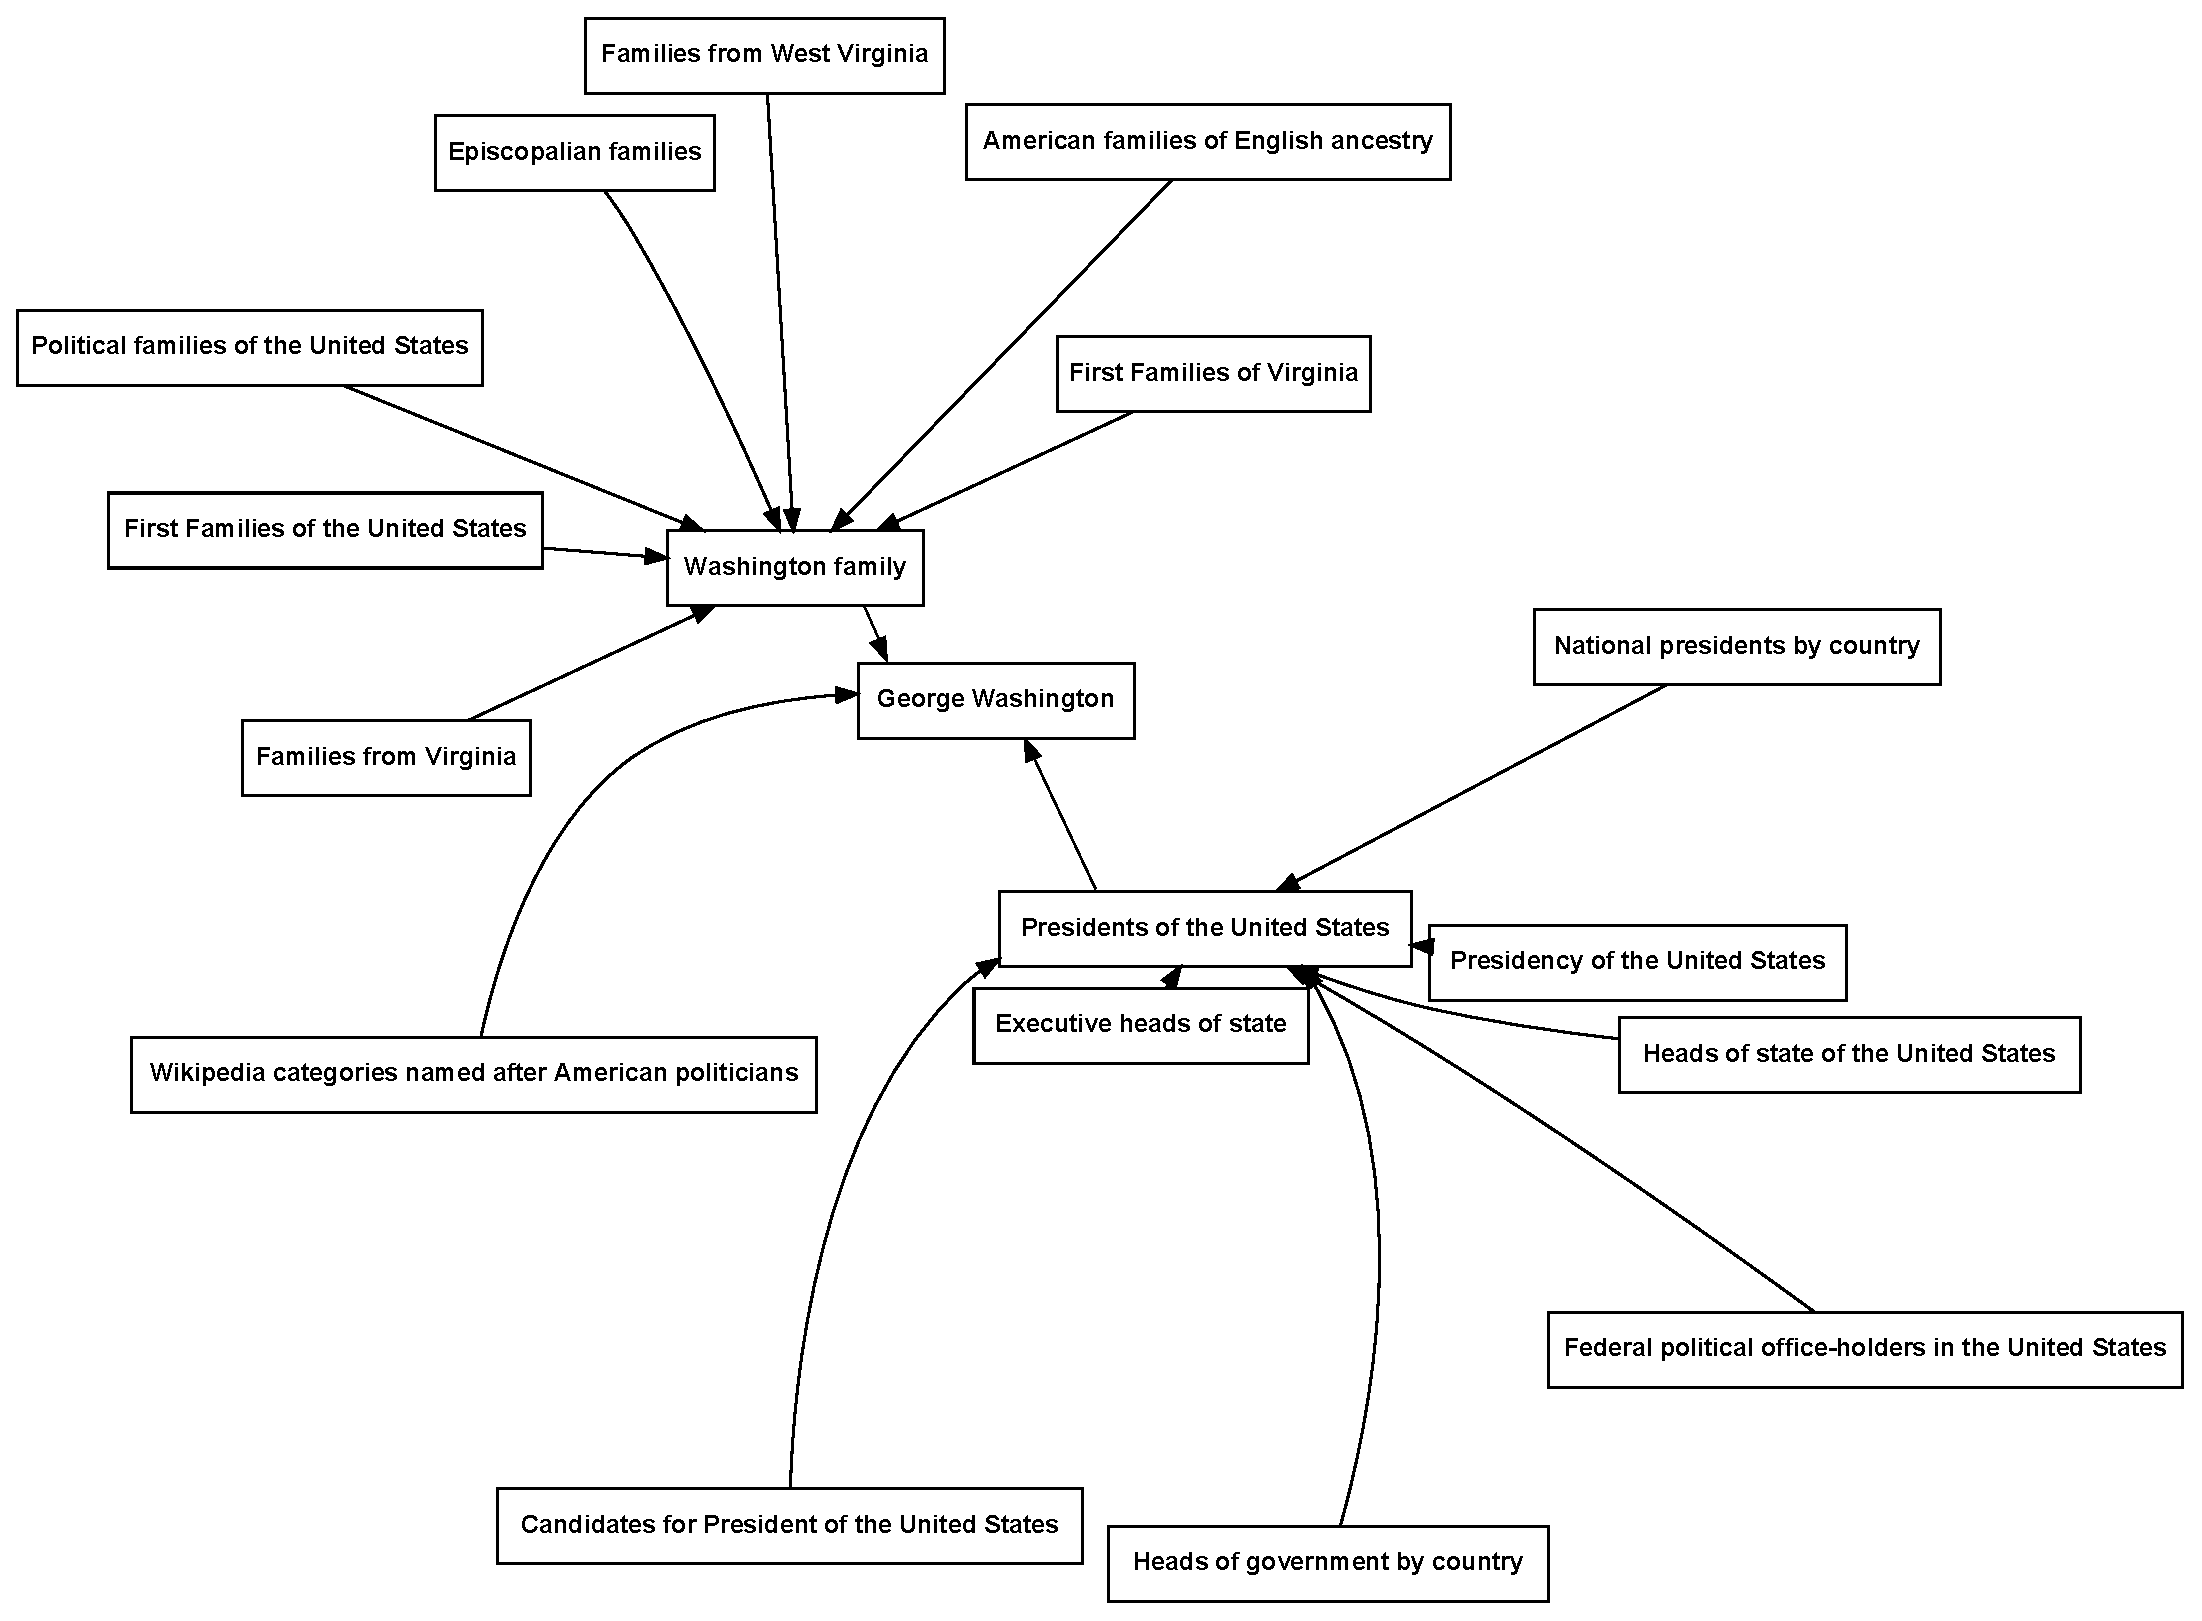
\includegraphics[width=1.0\linewidth]{washington-graph}
	\end{center}
	\vspace{-12pt}
	\caption{A small part of the category heirarchy for the Wikipedia article on ``George Washington''.}
	\label{fig:washington-graph}
\end{figure*}


\section{Related Work}
\label{sec:related_work}
Because Wikipedia is such a rich, diverse corpus of information, a lot of areas of machine learning research use Wikipedia as a training set for a variety of learned models. In this way, Wikipedia is used to improve the quality of machine learning research. This paper proposes the opposite: to use machine learning techniques to improve the quality of Wikipedia.

Automated classification of Wikipedia categories is an area that has been studied from several different angles. The category system contains a huge amount of extractable information, although it is very loosely structured~\cite{Ponzetto,Strube}. This loose structure arises naturally in Wikipedia, since articles are written and edited collaboratively. Furthermore, category links are not applied in a consistent or systematic manner across all of Wikipedia. The most simplistic approaches to categorizing Wikipedia utilize supervised learning. Supervised learning takes as input a set of training examples and their associated labels. In our case, these training examples are Wikipedia articles and their labels are the categories associated with them. Supervised learning uses these labeled training examples to learn a model which can predict the labels of previously unseen examples~\cite{Szymanski}.

There are two broad groups of features which are used as input to supervised learning algorithms: content features and network features. Content features reflect information directly contained within a given page. Examples of content features include textual keywords, infobox information, and metadata associated with a specific article~\cite{Tkachenko}. Network features describe the hyperlinked graph of Wikipedia articles and may contain information such as the number of outgoing links, the number of incoming links, and properties of neighbors in this hyperlinked graph~\cite{Getoor}.

The use of content features or network features alone has yielded impressive results~\cite{Gantner, Szymanski}. Using a combination of both feature types has been shown to be even more effective~\cite{Gantner}. Although supervised learning techniques are highly accurate for a few very specific categories~\cite{Gantner, Fu, Szymanski, Tkachenko}, they suffer from problems of scale. This is primarily because a classifier must be trained for each and every category. This approach will clearly not scale across the entire category system of Wikipedia, with its large and constantly changing set of categories~\cite{Fu}. Furthermore, previous work demonstrated that supervised learning is best for distinguishing between a few very distinct categories. This assumption does not hold across the vast majority of the category system, where categories may overlap or contain subtle differences~\cite{Thornton}. All of these limitations arise because supervised learning works primarily at the level of individually labeled articles, fundamentally limiting the amount of information that can be incorporated from the entire Wikipedia graph, even when network features are included.

Another approach to categorizing Wikipedia is to use semi-supervised learning algorithms. Semi-supervised learning differs from supervised learning in that it uses unlabeled data in the learning process. Many of these methods rely on label-propagation across a graph. The input to a semi-supervised learning algorithm is generally a set of examples. This set of examples is divided into labeled and unlabeled data. Using the assumption that the data are distributed in a way which correlates with their labels, the missing labels in the data can be estimated~\cite{Carlson}.

Azran~\cite{Azran} describes a generic example of an algorithm---known as the rendezvous algorithm---which can estimate a multi-class distribution of labels across examples. The rendezvous algorithm works by treating each example as a node in a fully connected graph. Each edge in this graph has an associated weight which is given by its entry in a pairwise similarity matrix between all examples called the transition matrix. Labeled example nodes are set to be absorbing states and unlabeled example nodes are set to be emitting states in a Markov random walk.  This means that each unlabeled example will emit a particle that chooses a neighbor to move to based on the probabilities defined in the transition matrix. At each new node, this particle chooses its next step based only on the probabilities defined for its current location---the ``Markov'' aspect of the random walk. Upon reaching a labeled node, the particle is absorbed and the label of the node is recorded. After running a number of random walks for each unlabeled node, the distribution of labels for that node can be inferred by looking at the distribution of absorbing states for its random walks.

Chidlovskii describes the results of a related random walk algorithm on Wikipedia. One of the important concerns he raises is the difficulty of computing a pairwise similarity matrix for a dataset as large as Wikipedia. One way to avoid this problem is to use the graph of hyperlinks between pages as a starting point for the transition matrix. Although the specifics of Chidlovskii's algorithm differ from the rendezvous algorithm, they demonstrate that label-propagation approaches have enormous potential in sparse graph applications such as Wikipedia~\cite{Chidlovskii}.

Graph based approaches such as these avoid the scalability bottleneck of needing to train an individual classifier for each category on Wikipedia. Furthermore, they allow us to incorporate all of the information inherent in the hyperlink structure of Wikipedia in our inference~\cite{Avrachenkov}. This link structure between articles has been found to be very highly correlated with the link structure of categories~\cite{Ponzetto, Holloway}, leading us to believe that it will be quite useful.

This paper plans to build on the preliminary results described here to develop a label propagation technique which can scale to the entire Wikipedia dataset. This approach will combine the robust, multiclass nature of a technique like the rendezvous algorithm with approaches for dealing with scalability similar to those Chidlovskii describes to produce a superior classification system.

\section{System Model}
\label{sec:system_model}
Our approach to this problem is twofold: first prune the input data to a more reasonable subset of potential article-category pairings. Then apply machine learning techniques using features inherent in each pairing to create a decision tree or other classifier which outputs a confidence in the correctness of the missing link. We then plan to integrate these results into a browser-based plugin which can provide a ranked list of the potential categorizations to editors as they browse through Wikipedia.

We will first generate rough suggestions by running a graph-based ``first-pass'' algorithm, which will provide potential missing categorizations in a graph of articles. The final result should exhibit high recall while still significantly reducing the number of possible categorizations for an article~\cite{Avrachenkov}. These potential article-category pairings will be used later as a basis for feature selection.

Next we take a statistically sampled subset of these potential categorizations and have individuals---ideally Wikipedia editors themselves, if we can recruit them---label each article-category pair as either good or bad. We plan to use the machine learning software Weka~\cite{Weka} to create a model for scoring and ranking the suggestions we have obtained from our graph-based approach. While high-recall was the goal of the graph-based algorithms, here we want to improve the precision of the suggestions we will ultimately produce. 

One important factor in learning such a model is determining the features that go into the algorithm. One feature that we will input to the algorithm is the numerical score from the graph algorithm. Other features that we will explore will include document similarity measures between an article and articles with the suggested category, metadata about the article and suggested category, and possibly properties of the category graph such as subcategory or supercategory relationships.

Finally if time allows and our techniques are robust enough we plan to make our data available to editors by integrating with the popular tool HotCat~\cite{HotCat}---which eases category management for Wikipedians. It is our plan to offer a simple ranked list of the top five or so potential categorizations for an article such that an editor visiting a page can quickly glance at our tool and check whether any of the supplied categories are appropriate. Figure~\ref{fig:block_diagram} illustrates the proposed architecture of the entire system in block-diagram form.
\begin{figure*}[htb!]
	\begin{center}
		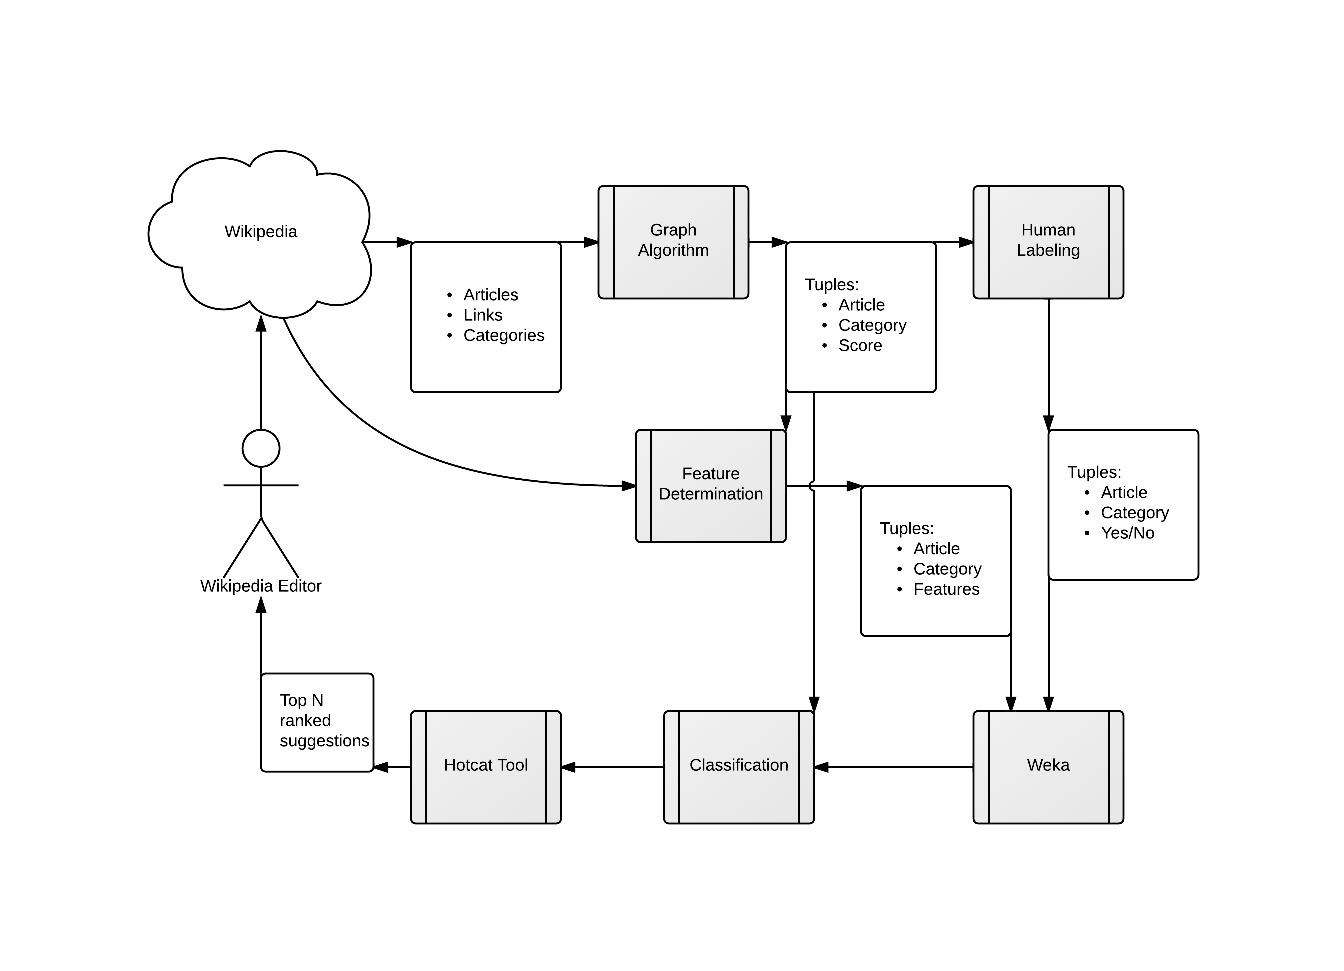
\includegraphics[width=1.0\linewidth]{block_diagram}
	\end{center}
	\vspace{-12pt}
	\caption{Our proposed system architecture. Gray blocks are processes, while arrows and white blocks represent data interchance between components.}
	\label{fig:block_diagram}
\end{figure*}

\section{System Implementation}
\label{sec:system_implementation}

Thus far we have completed implementation of the graph-based first phase. We chose Java as our primary language due to its acceptable performance for general computing tasks as well as our past experience using Java in large projects. Another consideration in choosing Java is the large number of libraries available as well as the possibility of using a distributed computing framework like Hadoop in the future.

Initially we planned to represent Wikipedia articles and categories as a graph-structure which could be contained entirely in memory. However, because all of the data we need is available as database tables this was unnecessary. These tables are available as SQL and can be obtained directly from Wikipedia. We chose to implement a system which uses calls to a mySQL database to lazy load articles and links as they are needed. For example, when our algorithm needs to find all outgoing links from an article, it queries a manager object which maintains a cache of all previously loaded pages and loads required pages on cache misses. This results in very little memory overhead for our running processes and a minimal number of queries to the database.

We have used this framework to build and test two different types of graph algorithms. Both algorithms take as input a specific article and return a list of potential new categories. One of the algorithms also outputs a score for each new category. These scores roughly correspond to the categories' relative frequency of occurrence in the input article's hyperlinked neighbors.

The first technique is a simple breadth-first search of all hyperlinked articles. This search returns the first n categories it finds, where n can be specified by the algorithm. Starting from a root article, the breadth-first search inspects the first adjacent (hyperlinked) article's categories and adds them to the output set of suggestions. This process is repeated in a breadth-first manner until the specified number of new categories are found. While this technique is fairly simple to implement, it does not output scores for each new category..

The second technique utilizes random walks to find and return a weighted score for new category suggestions. Starting from a root article, the algorithm queries all of its hyperlinked neighbors. The random walk currently has an equal probability of jumping to any of these neighbors. For walks of length greater than one, this process is repeated multiple times for each article jumped to. When a random walk has completed a number of jumps equal to its length, it adds the categories of the article it ended on to the output set of suggestions for the root article.

This technique runs a fixed number of iterations for each article. Each iteration currently performs a walk of length one, two, and three. A count of all new categories returned at the end of each walk is maintained. In order to weight categories that are farther from the root node lower, counts are incremented at a rate inversely proportional to their distance from the article. For example, seeing a category at distance three is worth one third of the weight of a category at distance one. At the end of all the iterations each category is given a final weight consisting of its count divided by the sum of all category counts. The results are then sorted and returned as suggestions.

One issue we have encountered is the inclusion of many administrative pages and categories in our results. While Wikipedia has an easy method for distinguishing administrative articles from informational articles, no such method exists for categories. We have filtered out administrative articles by ignoring anything not in the default namespace. Administrative categories are more difficult to filter, as there is no explicit identifier for them in the database tables provided by Wikipedia. We have been examining heuristics that take advantage of the relatively straightforward Wikipedia naming conventions for administrative categories. For example, one can usually safely ignore categories which begin with ``Articles\_with'', ``Articles\_lacking'', ``Articles\_needing'', or ``All\_articles\_with''.

\section{System Performance}
\label{sec:system_performance}

\subsection{Desired Properties}
\label{subsec:desired_properties}
Since our next milestone is to have annotators label a sample of good and bad category suggestions for articles, the desired properties of the of the graph algorithm are focused on efficiently generating a manageable list of recommendations. Therefore, the algorithm must have at least the following properties:
\begin{itemize*}
	\item {\sc High Recall}: Because the output from this algorithm will later be filtered by a classifier or machine-learned model, it is important that this phase of the project returns as many correct categories as possible. Poor categories can be filtered out later, but additional good suggestions cannot be generated after this stage.
	\item {\sc Scalable Performance}: Wikipedia is a vast dataset containing millions of articles which need categorization. This graph-based portion of the project works directly on each of these articles and their neighbors, meaning it will likely be the bottleneck for the entire system. Our tests on individual categories or small groups of categories must be able to scale to all of Wikipedia.
\end{itemize*}
Two additional, though not strictly required properties are listed below:
\begin{itemize*}
	\item {\sc Confidence Scores}: A confidence score would be a valuable input to building a model to classify suggestions as good or bad. This would also probably expedite the labeling process, since only the most relevant suggestions could be presented to annotators for labeling.
	\item {\sc Removal of Irrelevant Results}: As previously mentioned, removal of administrative pages and categories would reduce the number of pages requiring subsequent classification, as well as reduce noise in subsequent classification attempts. This could be performed in the classification phase of the project, but incorporating information from this graph-based approach may also prove helpful for removing irrelevant results.
\end{itemize*}
With these properties in mind, we have collected some preliminary results to guide our future efforts as the project progresses.

\subsection{Recall}
\label{subsec:recall}

\begin{table*}[htb!]
\centering
\begin{tabular}{|l|l|}
	\hline
	\multicolumn{1}{|c}{Random Walk} & \multicolumn{1}{|c|}{Breadth-First-Search} \\ \hline
	port\_cities\_and\_towns\_of\_the\_baltic\_sea&knights\_of\_the\_golden\_fleece\\ \hline
	academy\_honorary\_award\_recipients&denmark\_norway\\ \hline
	translators\_from\_danish&history\_of\_santa\_barbara\_county,\_california\\ \hline
	cecil\_b\_demille\_award\_golden\_globe\_winners&use\_dmy\_dates\_from\_august\_2011\\ \hline
	copenhagen&1768\_births\\ \hline
	municipal\_seats\_in\_capital\_region\_of\_denmark&danish\_american\_history\\ \hline
	danish\_silent\_film\_actors&extra\_knights\_companion\_of\_the\_garter\\ \hline
	use\_dmy\_dates\_from\_august\_2012&regions\_of\_italy\\ \hline
	american\_people\_of\_danish\_descent&characters\_in\_fairy\_tales\\ \hline
	translators\_to\_english&dukes\_of\_schleswig\\ \hline
\end{tabular}
\caption{Recall Data}
\end{table*}

\subsection{Scalable Performance}
\label{subsec:scalable_performance}

\section{Remaining Work}
\label{sec:remaining_work}


\bibliographystyle{plain}
\bibliography{proposal}
\nocite{*}

\end{document} 

